\documentclass{article}
\usepackage[utf8]{inputenc}

\title{Problem 1 (PI)}
\author{Baiyu Huo}
\date{July 2019}

\usepackage{natbib}
\usepackage{graphicx}
\usepackage{amsmath}

\begin{document}

\maketitle

\section{Description}
The number PI is a mathematical constant. It used to describe the ratio of the circles' circumference and its diameter, and nowadays it has been used by many formulas in both mathematics and physics. It is an Irrational number which means it can not be present as the ratio of two integers. What's more, PI is also a transcendental number, which means that "it is not the solution of any non-constant polynomial equation with rational coefficients".\citep{wiki:pi} It approximately equals to 3.141592653.


\begin{figure}[h!]
\centering
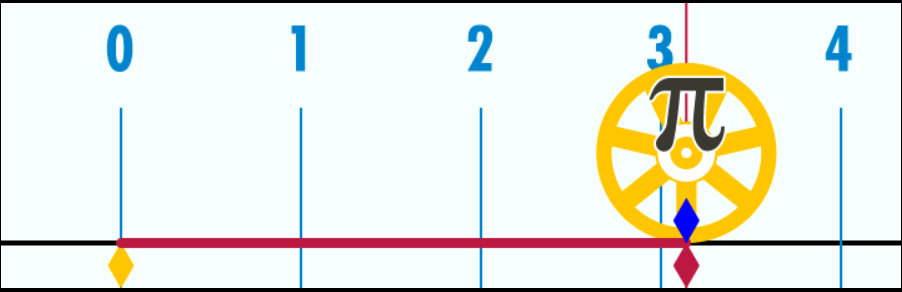
\includegraphics[scale=0.2]{PI.png}
\caption{PI}
\label{fig:universe}
\end{figure}

\paragraph{Difination}
let C equals circle's circumference, d equals circle's diameter, then PI equals the radio of C and d.


\begin{center}
 $PI=\frac{C}{d}$
\end{center}

\paragraph{Usage} 
Geometry and trigonometry, Eigenvalues, Inequalities, Fourier transform and Heisenberg uncertainty principle, Gaussian integrals,Projective geometry, Topology etc.



\bibliographystyle{plain}
\bibliography{references}
\end{document}


